\documentclass[12pt]{article}

\usepackage{geometry}
 \geometry{
 a4paper,
 total={170mm,257mm},
 left=20mm,
 right=10mm,
 top=45mm,
 bottom=20mm,
 headheight=75pt
 }
% \usepackage[utf8x]{inputenc}
\usepackage{fontspec}
\setmainfont{Open Sans}
\setsansfont{Noto Sans}
\usepackage{graphicx}
\usepackage{subcaption}
\usepackage{url}       % `\url`s
\usepackage{floatrow}
\usepackage{hyperref}
\usepackage{cleveref}
\graphicspath{{resources_CAE/}}

\usepackage{fancyhdr}
\pagestyle{fancy}


\renewcommand{\headrulewidth}{0pt}
\fancyhead[C]{\LARGE <<Introduction to Mechanical Engineering>> \\ \textbf{Final Exam} \\ \textit{CAE part} \\ Variant: \thepage}
\fancyfoot[]{}


\newcommand\pic[1]{(\cref{#1})} %Где нужно сослаться на рисунок

\hypersetup{
    colorlinks=true,
    linkcolor=blue,
    urlcolor=cyan,
    }

\newcommand\ttask[3] 
 {
	\section*{#1}
	\textbf{Input data description}: \\ #2 \  \\
	\textbf{Task description description}: #3
	\newpage
 }

% The preamble ends with the command \begin{document}
\begin{document} % All begin commands must be paired with an end command somewhere

\ttask{Rifle simulation}{Create a simplified geometric model of the bullet in the barrel of the rifle at the moment of firing \pic{fig:var1_0.jpeg}. Approximate parameters of the model:
	\begin{itemize}
		\item Bullet weight: 9 g.
		\item Barrel weight: 250 g.
		\item Gunpowder combustion force: 500 N.
		\item Powder combustion time: 0.01 s.
	\end{itemize}}{
	\begin{itemize}
		\item Check the law of conservation of momentum at the moment of firing. Give graphs of the velocity of the bullet and the barrel --- \pic{fig:var1_1.jpeg}.
		\item Determine the velocity of the bullet at the moment of departure from the barrel.
		\item Calculate (experimentally) the spring stiffness \pic{fig:var1_0.jpeg} , which should bring the striker to its initial state in about 0.02 seconds after the shot. Give a graph of the movement of the striker at the moment of firing \pic{fig:var1_2.jpeg}. Determine the "recoil distance" of the striker.
	\end{itemize}

	\begin{figure}[H]
		\begin{subfigure}{0.5\textwidth}
			\centering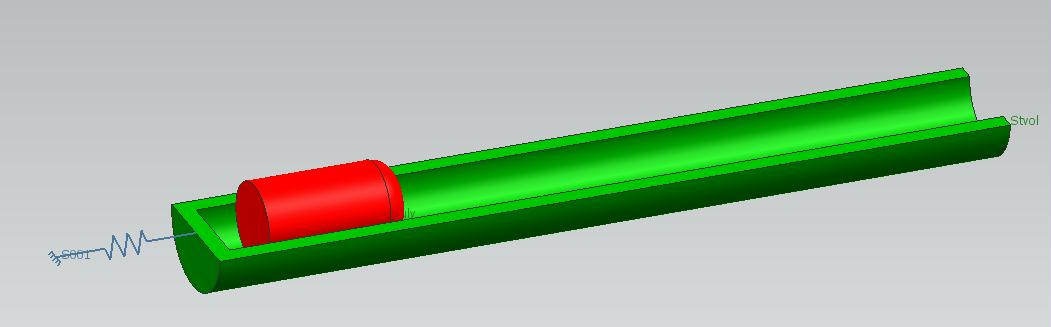
\includegraphics[height=6cm,width=1\textwidth,keepaspectratio]{var1_0.jpeg}
			\caption{}
			\label{fig:var1_0.jpeg}
		\end{subfigure}

		\begin{subfigure}{0.49\textwidth}
			\centering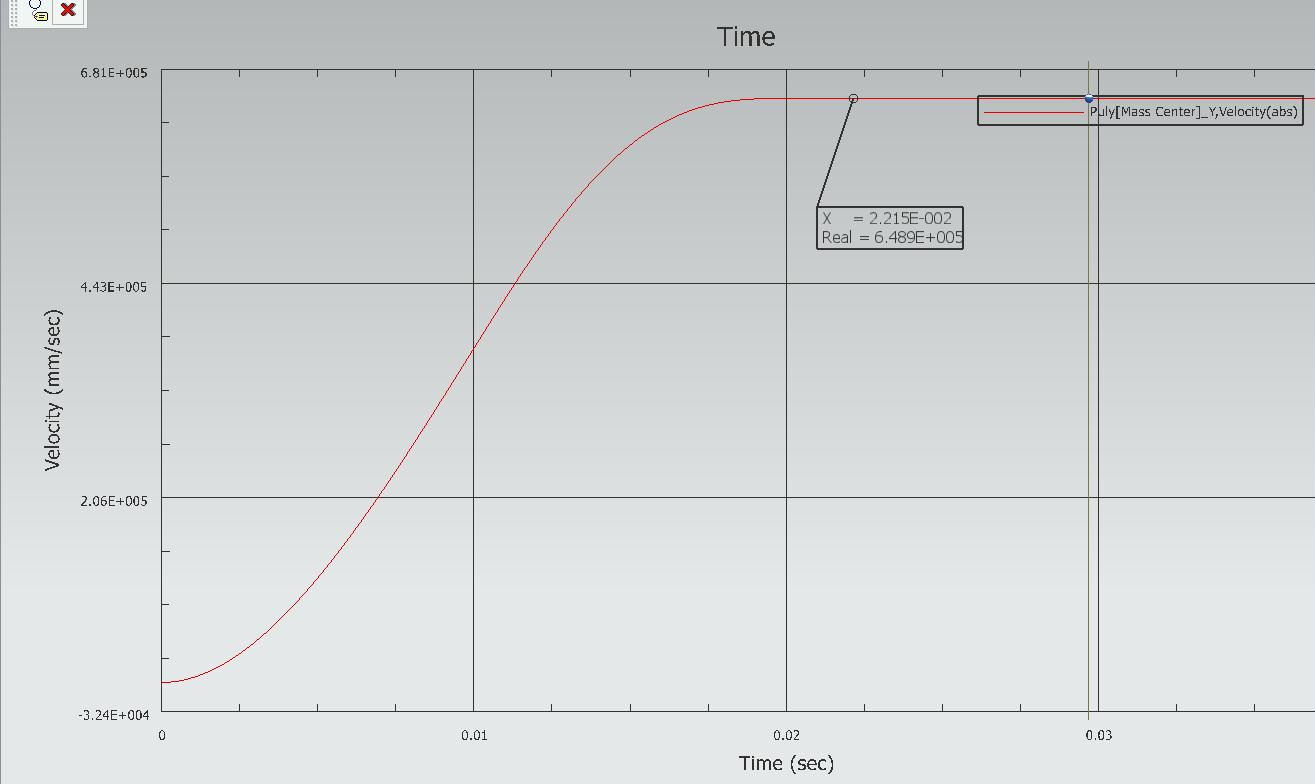
\includegraphics[height=5cm,width=1\textwidth,keepaspectratio]{var1_1.jpeg}
			\caption{}
			\label{fig:var1_1.jpeg}
		\end{subfigure}
		\begin{subfigure}{0.49\textwidth}
			\centering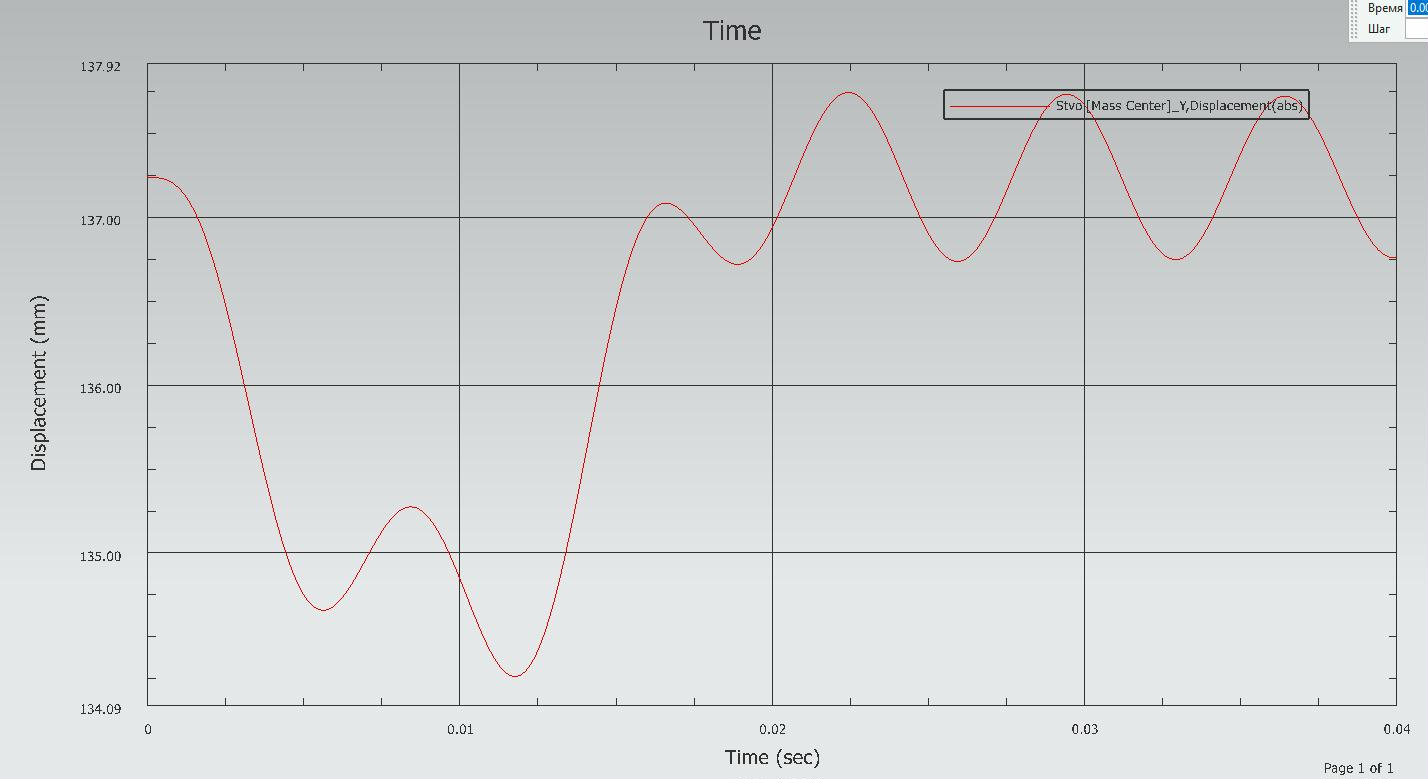
\includegraphics[height=5cm,width=1\textwidth,keepaspectratio]{var1_2.jpeg}
			\caption{}
			\label{fig:var1_2.jpeg}
		\end{subfigure}
	\end{figure}
}

\ttask{Waterwheel}{
	Create a geometric model of the water wheel (\cref{fig:var2_0.jpeg}). The mass of the wheel is approximately 650 kg.
}{
	\begin{itemize}
		\item Apply a single impulse force to one of its blades (\cref{fig:var2_1.jpeg}), which acts only for 0.1 - 0.15 seconds (\cref{fig:var2_2.jpeg}).
		\item Calculate or select the amount of force applied so that the wheel turns a quarter turn in about 2 seconds (\cref{fig:var2_3.jpeg}).
	\end{itemize}

	\begin{figure}[H]
		\begin{subfigure}{0.49\textwidth}
			\centering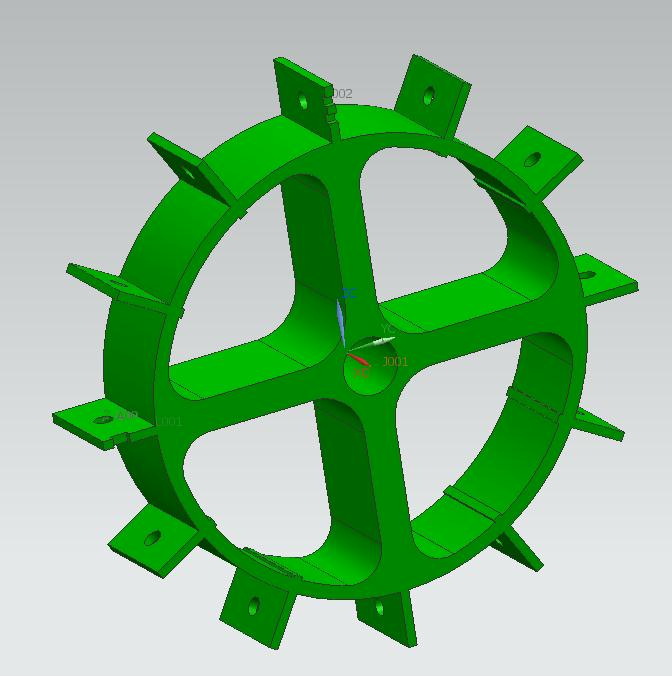
\includegraphics[height=6cm,width=1\textwidth,keepaspectratio]{var2_0.jpeg}
			\caption{}
			\label{fig:var2_0.jpeg}
		\end{subfigure}
		\begin{subfigure}{0.49\textwidth}
			\centering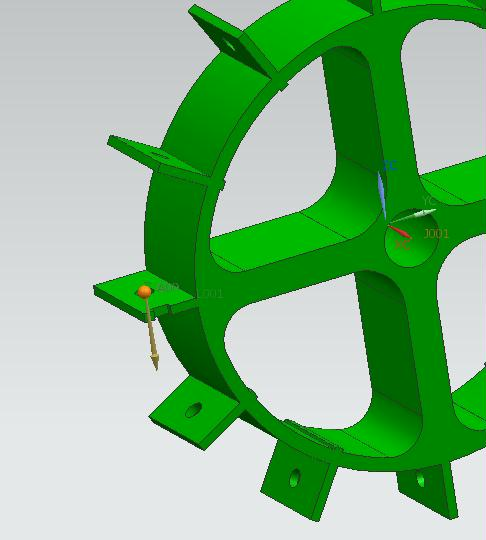
\includegraphics[height=6cm,width=1\textwidth,keepaspectratio]{var2_1.jpeg}
			\caption{}
			\label{fig:var2_1.jpeg}
		\end{subfigure}
	
		\begin{subfigure}{0.49\textwidth}
			\centering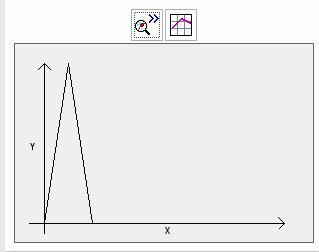
\includegraphics[height=6cm,width=1\textwidth,keepaspectratio]{var2_2.jpeg}
			\caption{}
			\label{fig:var2_2.jpeg}
		\end{subfigure}
		\begin{subfigure}{0.49\textwidth}
			\centering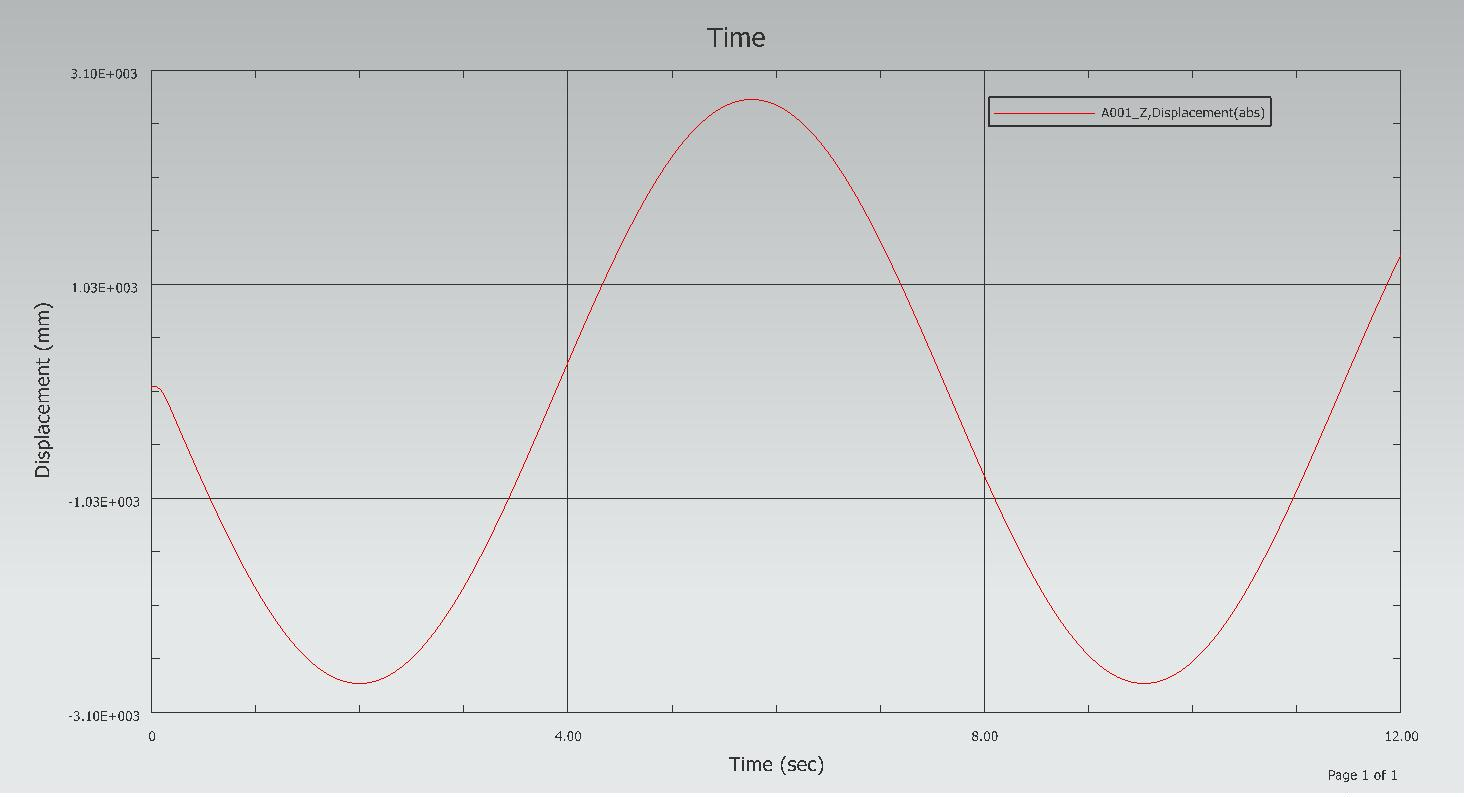
\includegraphics[height=6cm,width=1\textwidth,keepaspectratio]{var2_3.jpeg}
			\caption{}
			\label{fig:var2_3.jpeg}
		\end{subfigure}
	\end{figure}
}

\ttask{Modified moment of inertia}{
	Create a geometric model of a simple mechanism (\cref{fig:var3_0.jpeg}). The mass of the gray base is about 1 kg. The mass of the red weight is about 0.7 kg. The red weight can only move along the gray sled. The base rotates around fix based by external torque (approx 2000 Nmm)
}{
	You should solve the task for 2 cases.
	\begin{enumerate}
		\item The red weight remains in place during rotation (for this purpose it is placed strictly in the middle), the angular velocity of the entire structure is constantly increasing.
		\item The red load is somewhat shifted to the side (\cref{fig:var3_1.jpeg}), then during rotation of the gray base, this load will "move away" under the action of centrifugal force, and because of the increased moment of inertia of the whole structure, the movement will quickly stop. In the figure (\cref{fig:var3_2.jpeg}) shows a graph of angular velocity of the whole structure for this case.
	\end{enumerate}
	The task is to determine the maximum angular velocity of the structure that will be reached and the point in time when this maximum will occur.

	\begin{figure}[H]
		\begin{subfigure}{0.42\textwidth}
			\centering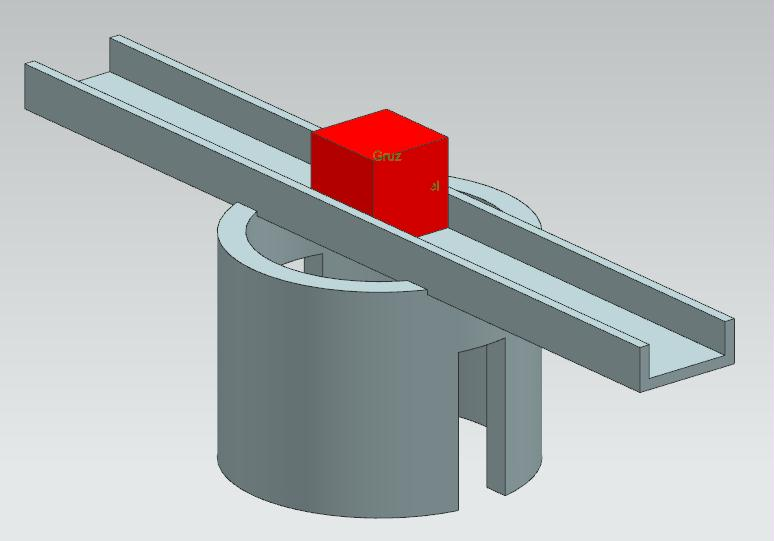
\includegraphics[height=6cm,width=1\textwidth,keepaspectratio]{var3_0.jpeg}
			\caption{}
			\label{fig:var3_0.jpeg}
		\end{subfigure}
		\begin{subfigure}{0.42\textwidth}
			\centering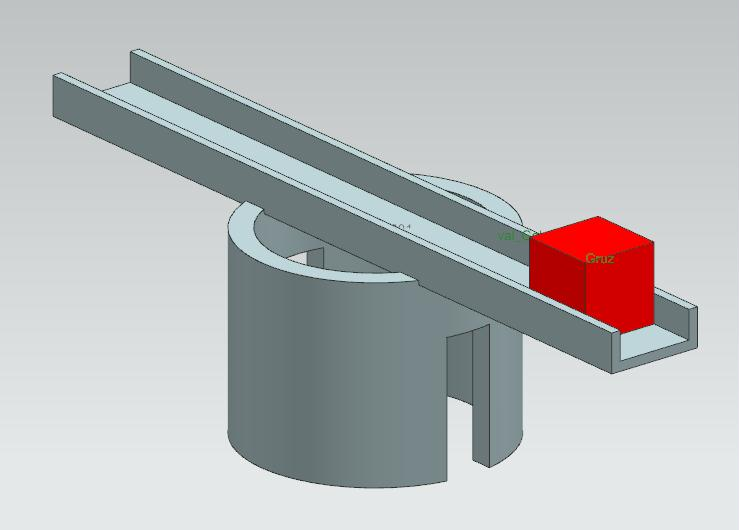
\includegraphics[height=6cm,width=1\textwidth,keepaspectratio]{var3_1.jpeg}
			\caption{}
			\label{fig:var3_1.jpeg}
		\end{subfigure}

		\begin{subfigure}{0.8\textwidth}
			\centering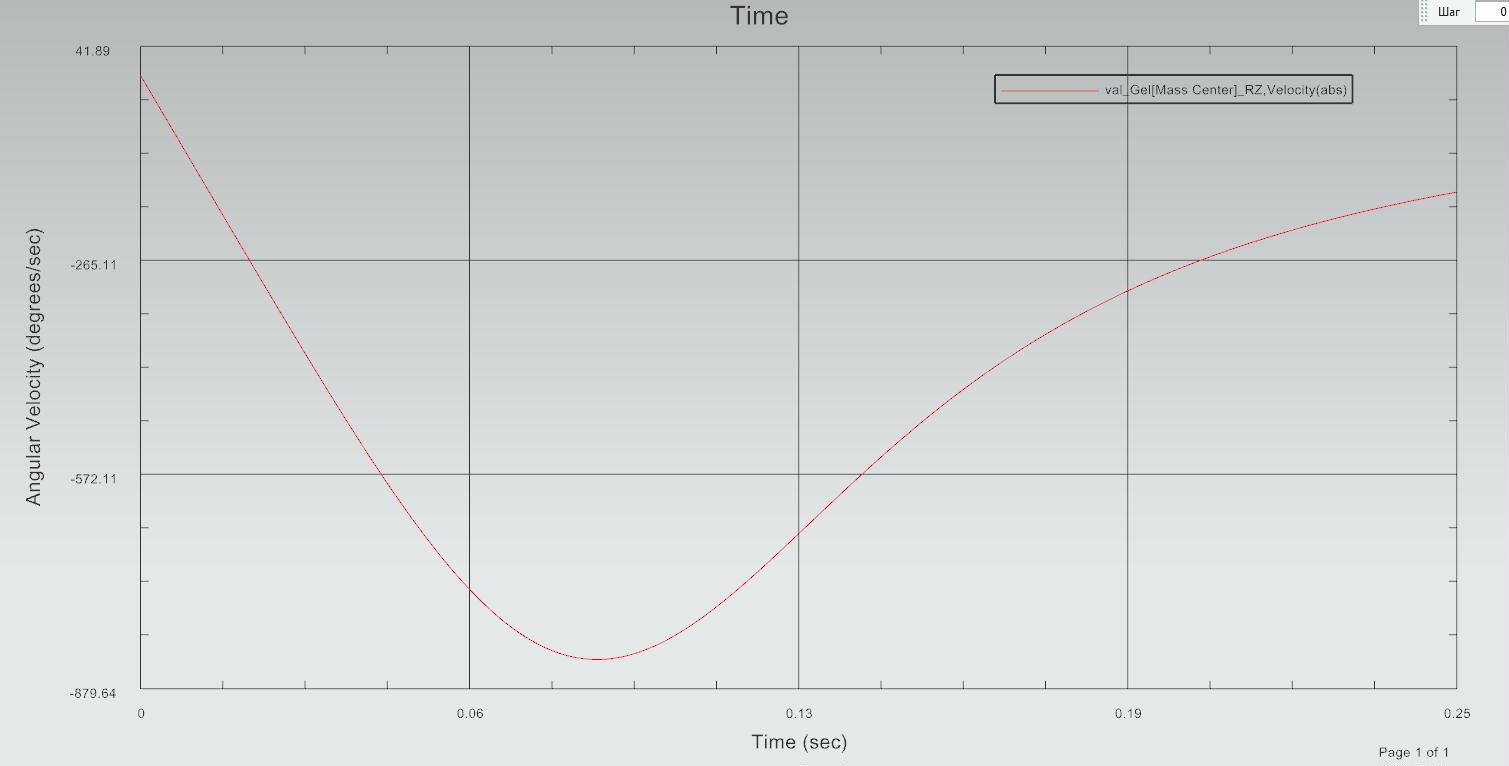
\includegraphics[height=6cm,width=1\textwidth,keepaspectratio]{var3_2.jpeg}
			\caption{}
			\label{fig:var3_2.jpeg}
		\end{subfigure}
	\end{figure}
}

\ttask{Centrifugal force of flywheel}{
	Construct a geometric model of a simple mechanism (\cref{fig:var4_0.jpeg}). The geometry of the red flywheel can be completely arbitrary (but flat). The red flywheel swings by its own weight.
}{
	\begin{itemize}
		\item Determine the necessary mass-inertia characteristics of the red flywheel.
		\item Plot the reactive force in the rotational joint (\cref{fig:var4_1.jpeg}).
		\item Plot the linear velocity of the center of mass of the flywheel (\cref{fig:var4_2.jpeg}).
		\item Find the centrifugal force by $F= \frac{m v^2}{r}$, where $m$ --- flywheel mass, $v$ --- linear velocity of the flywheel, $r$ --- center of mass swing radius of the flywheel.
		\item Show that at a certain point in time the reactive force in the rotational joint is the weight of the flywheel, plus its centrifugal force.
	\end{itemize}

	\begin{figure}[H]
		\begin{subfigure}{0.5\textwidth}
			\centering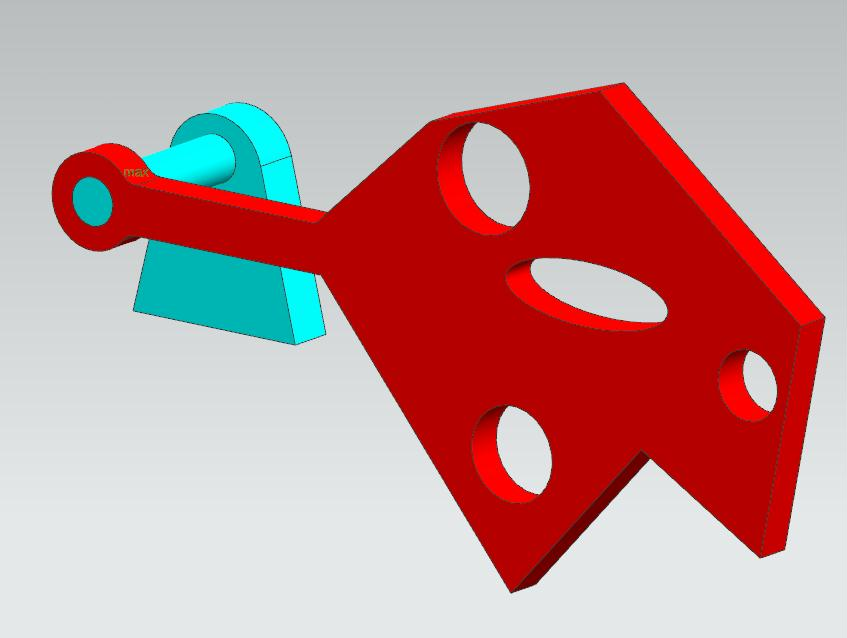
\includegraphics[height=6cm,width=1\textwidth,keepaspectratio]{var4_0.jpeg}
			\caption{}
			\label{fig:var4_0.jpeg}
		\end{subfigure}

		\begin{subfigure}{0.49\textwidth}
			\centering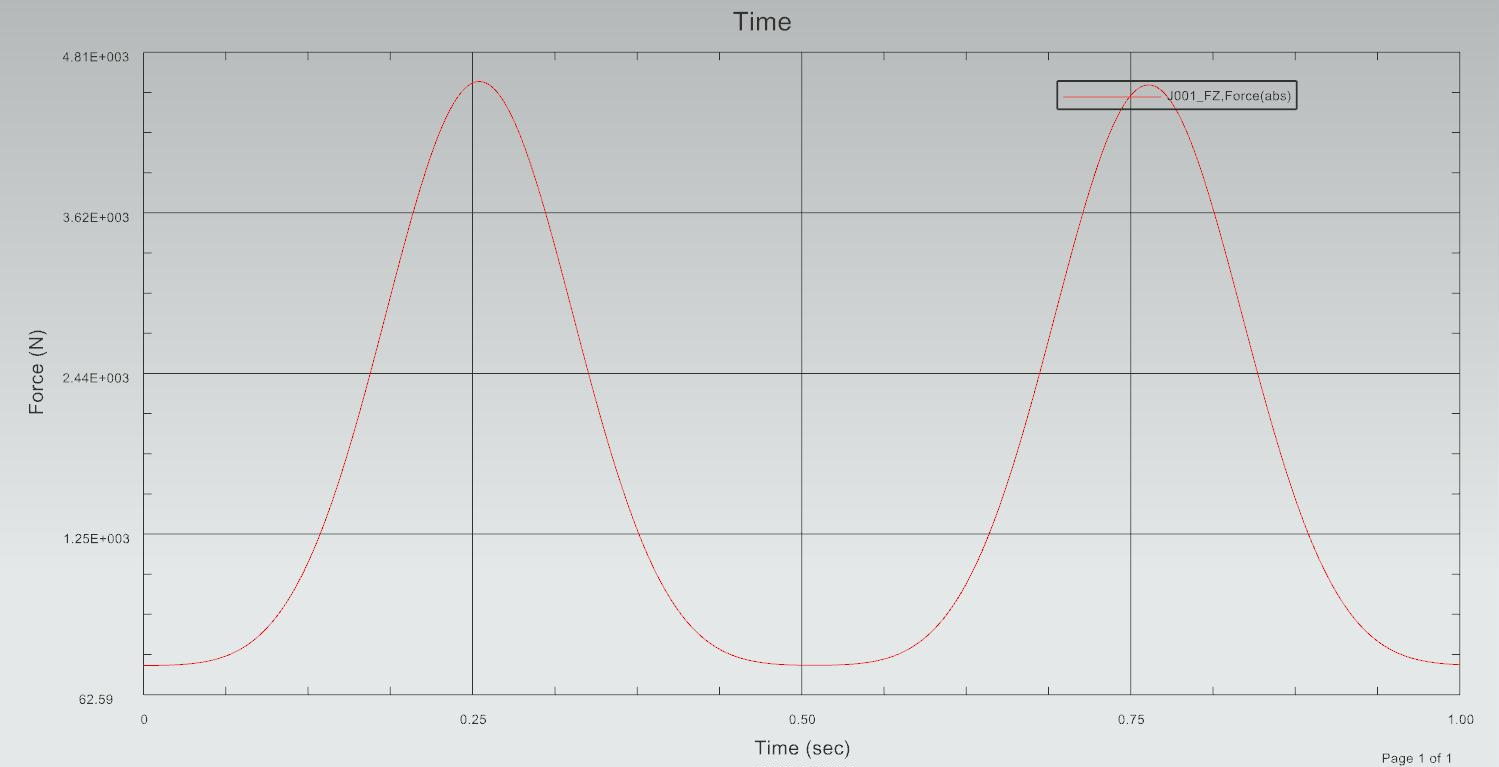
\includegraphics[height=6cm,width=1\textwidth,keepaspectratio]{var4_1.jpeg}
			\caption{}
			\label{fig:var4_1.jpeg}
		\end{subfigure}
		\begin{subfigure}{0.49\textwidth}
			\centering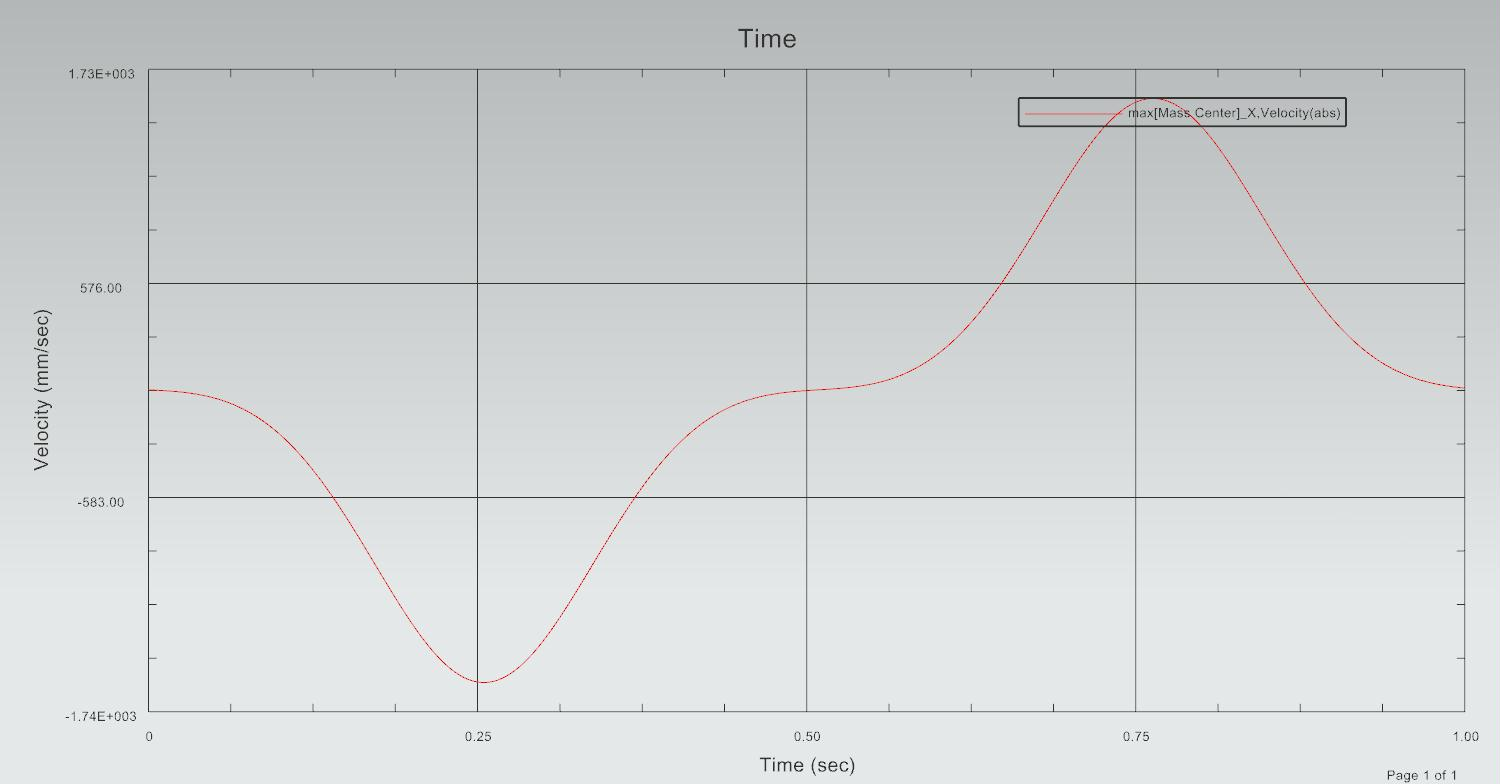
\includegraphics[height=6cm,width=1\textwidth,keepaspectratio]{var4_2.jpeg}
			\caption{}
			\label{fig:var4_2.jpeg}
		\end{subfigure}
	\end{figure}
}

\ttask{Flywheel acceleration}{
	Create a geometric model of a simple mechanism (\cref{fig:var5_0.jpeg}) that simulates the acceleration of the green flywheel by the force applied to the blue piston. Combined weight of the wheel and connecting rod of about 30 to 40 kg.
}{
	\begin{itemize}
		\item For accelerating the flywheel, you should apply the periodic force (\cref{fig:var5_1.jpeg}). The magnitude of the force is 30 N.
		\item Plot the graphs of the applied force (\cref{fig:var5_1.jpeg}) and the angular velocity of the spinning wheel (\cref{fig:var5_2.jpeg}).
	\end{itemize}

	\begin{figure}[H]
		\begin{subfigure}{0.6\textwidth}
			\centering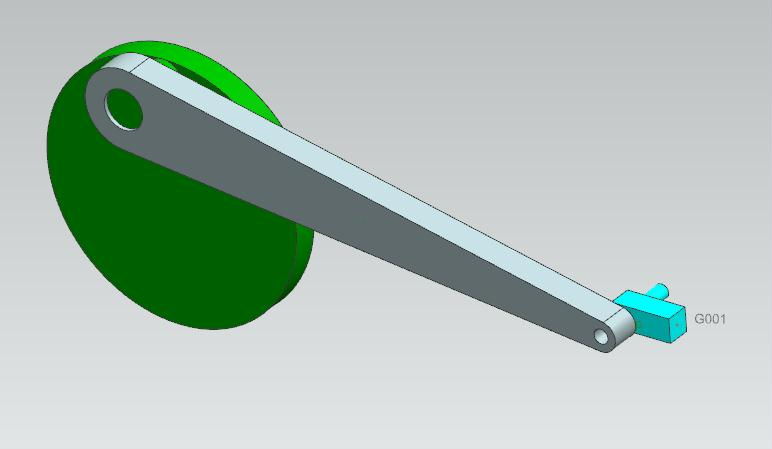
\includegraphics[height=6cm,width=1\textwidth,keepaspectratio]{var5_0.jpeg}
			\caption{}
			\label{fig:var5_0.jpeg}
		\end{subfigure}

		\begin{subfigure}{0.49\textwidth}
			\centering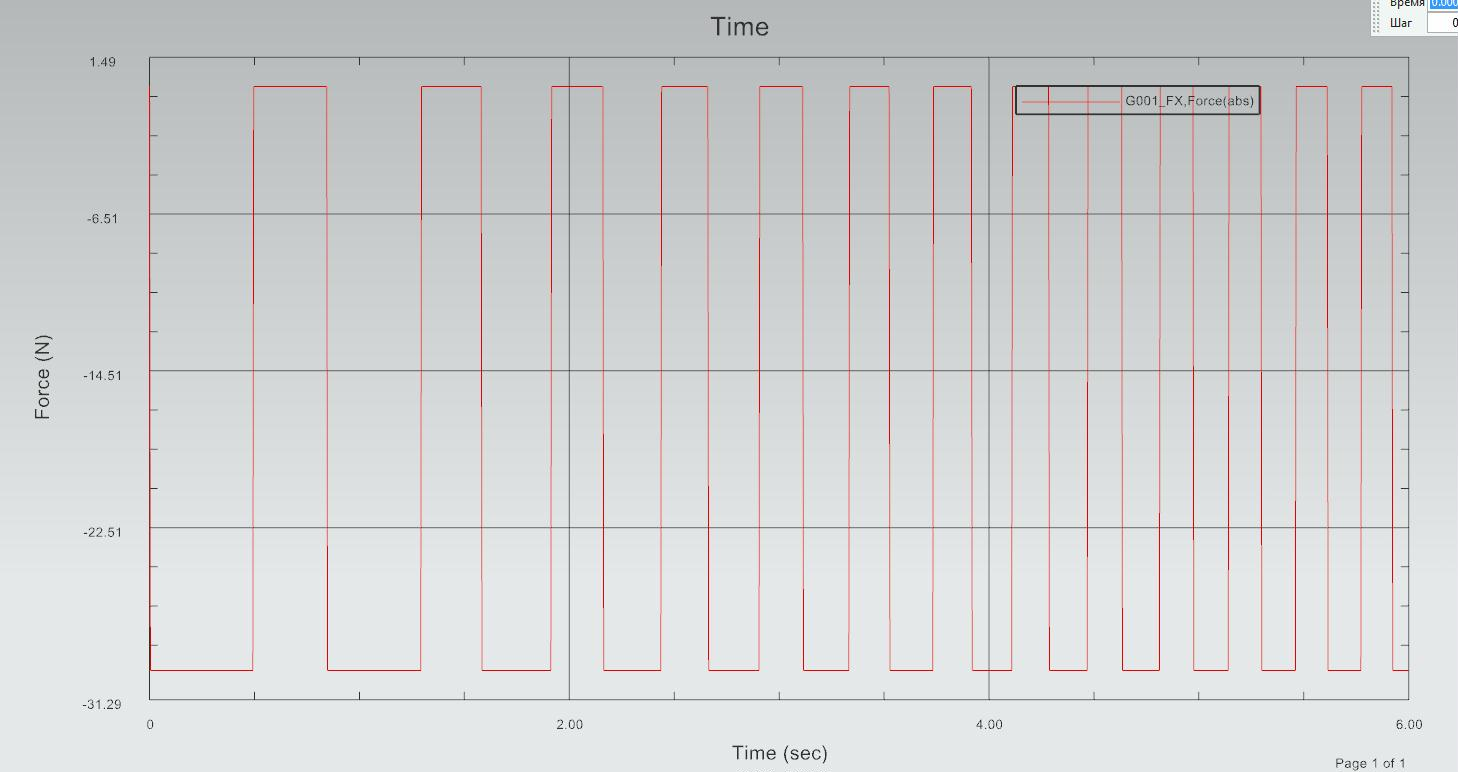
\includegraphics[height=6cm,width=1\textwidth,keepaspectratio]{var5_1.jpeg}
			\caption{}
			\label{fig:var5_1.jpeg}
		\end{subfigure}
		\begin{subfigure}{0.49\textwidth}
			\centering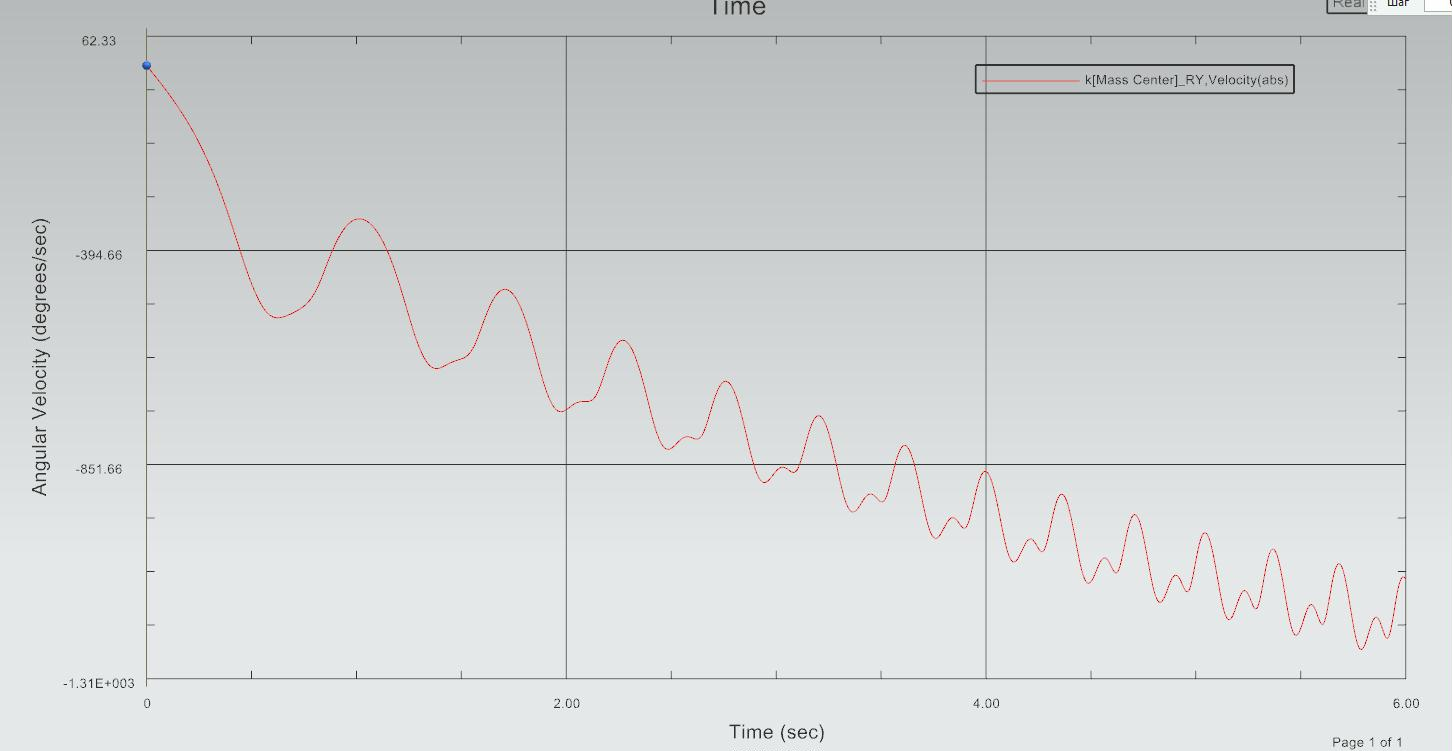
\includegraphics[height=6cm,width=1\textwidth,keepaspectratio]{var5_2.jpeg}
			\caption{}
			\label{fig:var5_2.jpeg}
		\end{subfigure}
	\end{figure}
}

\ttask{Monotonous pendulum stopping}{
	Construct a simple geometric model of the pendulum shown below (\cref{fig:var6_0.jpeg}). The mass of the red pendulum is approximately 1.5 - 2 kg.
}{
	\begin{itemize}
		\item Apply a monotonically acting force to the pendulum in such a way as to completely restrict its center of mass from entering the negative XC region. Thus, the position of the pendulum shown in \cref{fig:var6_1.jpeg} is considered to be completely unacceptable. To sum up, the force must constantly throw the pendulum to the right every time it reaches its vertical state. Its maximum possible entry into the negative XC region is shown in \cref{fig:var6_2.jpeg}.
		\item The applied force must be described by a special function. \cref{fig:var6_3.jpeg} shows a graph of a possible monotonic force. 
		\item Change the magnitude of the applied force from 10N to 110N. Show how this affects how much the pendulum goes into the negative XC region, and the length of time that the monotonic force will act (\cref{fig:var6_3.jpeg}).
	\end{itemize}
	\begin{figure}[H]
		\begin{subfigure}{0.49\textwidth}
			\centering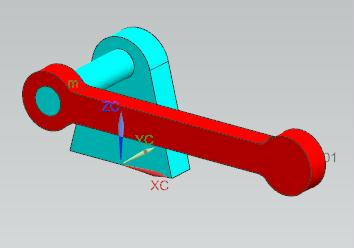
\includegraphics[height=4.5cm,width=1\textwidth,keepaspectratio]{var6_0.jpeg}
			\caption{}
			\label{fig:var6_0.jpeg}
		\end{subfigure}
		\begin{subfigure}{0.49\textwidth}
			\centering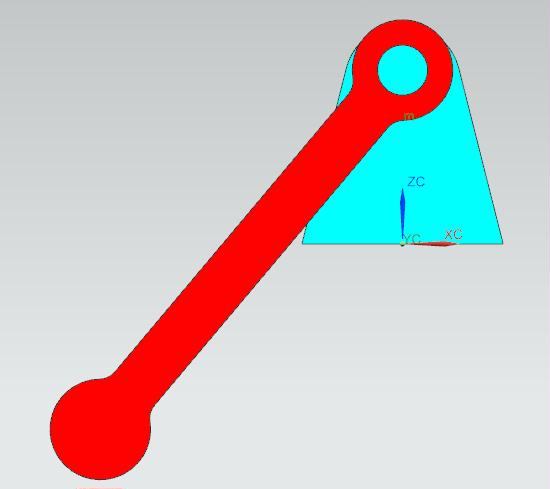
\includegraphics[height=4.5cm,width=1\textwidth,keepaspectratio]{var6_1.jpeg}
			\caption{}
			\label{fig:var6_1.jpeg}
		\end{subfigure}

		\begin{subfigure}{0.49\textwidth}
			\centering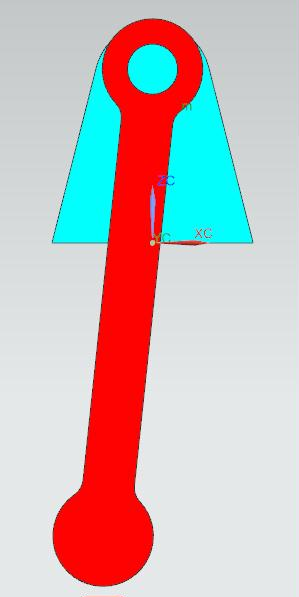
\includegraphics[height=6cm,width=1\textwidth,keepaspectratio]{var6_2.jpeg}
			\caption{}
			\label{fig:var6_2.jpeg}
		\end{subfigure}
		\begin{subfigure}{0.49\textwidth}
			\centering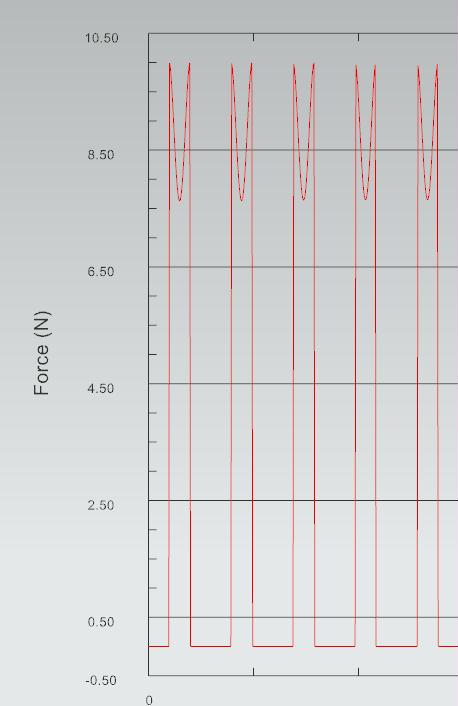
\includegraphics[height=6cm,width=1\textwidth,keepaspectratio]{var6_3.jpeg}
			\caption{}
			\label{fig:var6_3.jpeg}
		\end{subfigure}
	\end{figure}
}

\ttask{Billiards}{
	Create a geometric model of a billiard table with two balls on it (\cref{sub@fig:var7_0.jpeg}). The mass of the balls is approximately 500 g. The analysis time is 1 sec.
}{
	You should make that white ball hits a red ball, the latter hits the pocket (\cref{sub@fig:var7_1.jpeg,sub@fig:var7_2.jpeg,sub@fig:var7_3.jpeg,sub@fig:var7_4.jpeg}). It should be a tangential hit. It is impulse force.

	\begin{figure}[H]
		\begin{subfigure}{0.90\textwidth}
			\centering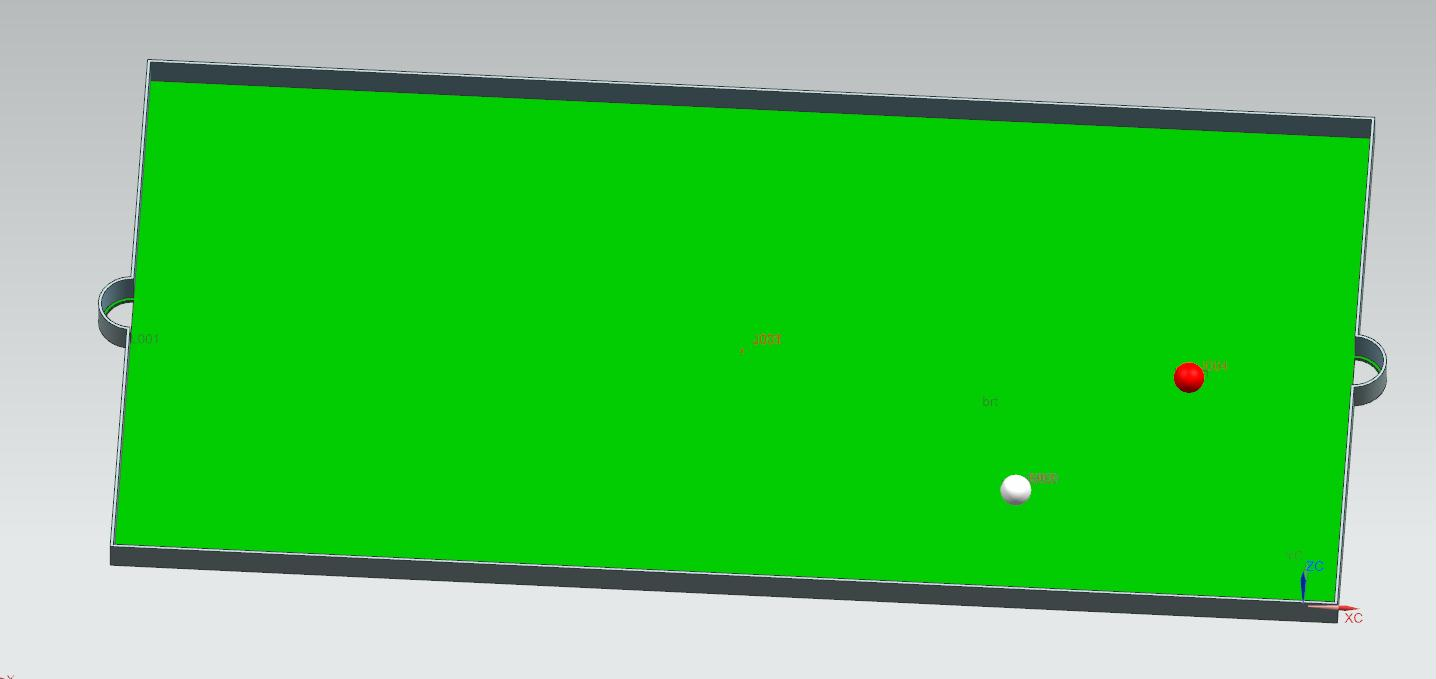
\includegraphics[height=6cm,width=1\textwidth,keepaspectratio]{var7_0.jpeg}
			\caption{}
			\label{fig:var7_0.jpeg}
		\end{subfigure}

		\begin{subfigure}{0.49\textwidth}
			\centering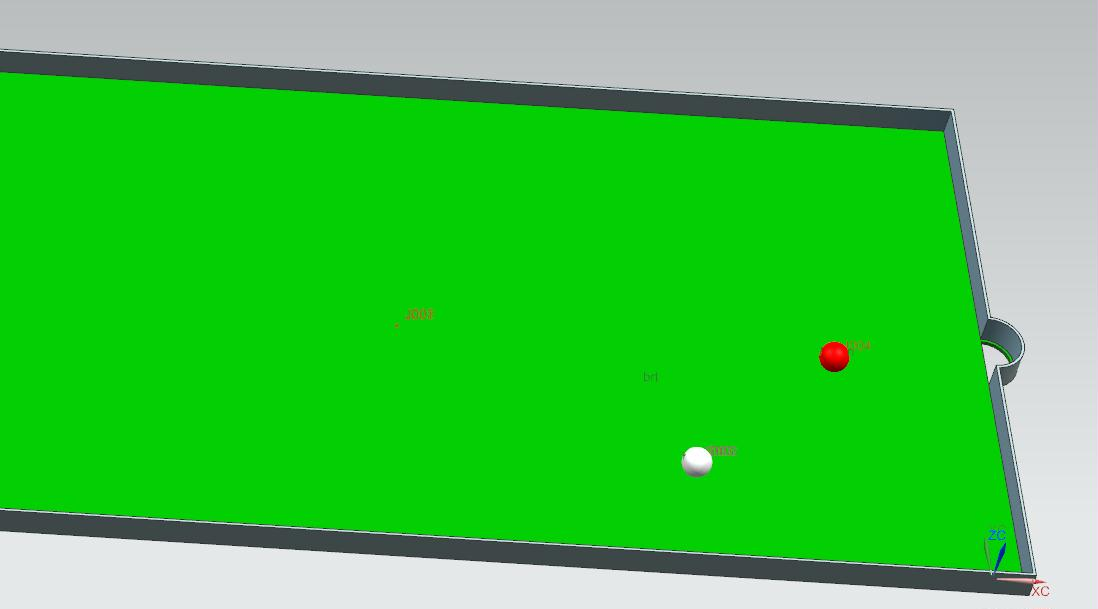
\includegraphics[height=5cm,width=1\textwidth,keepaspectratio]{var7_1.jpeg}
			\caption{}
			\label{fig:var7_1.jpeg}
		\end{subfigure}
		\begin{subfigure}{0.49\textwidth}
			\centering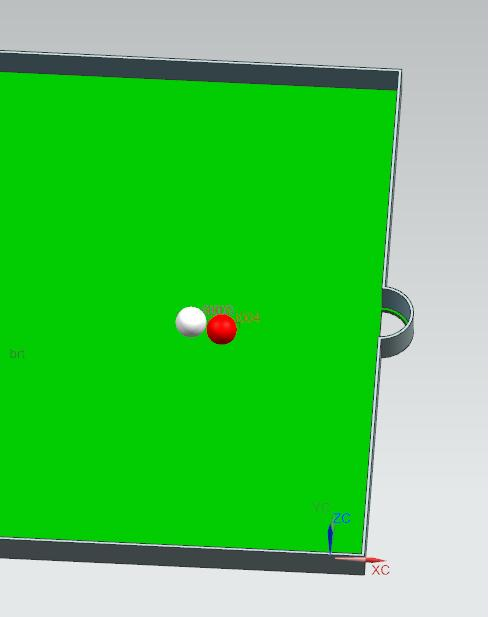
\includegraphics[height=5cm,width=1\textwidth,keepaspectratio]{var7_2.jpeg}
			\caption{}
			\label{fig:var7_2.jpeg}
		\end{subfigure}

		\begin{subfigure}{0.49\textwidth}
			\centering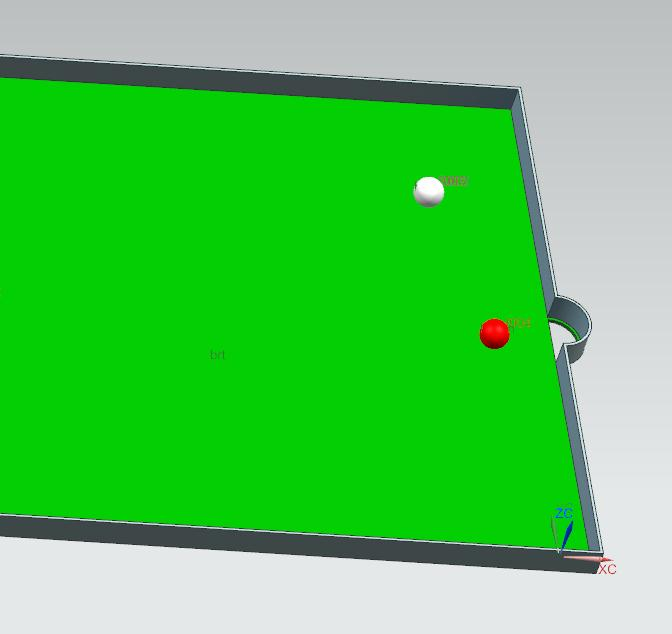
\includegraphics[height=5cm,width=1\textwidth,keepaspectratio]{var7_3.jpeg}
			\caption{}
			\label{fig:var7_3.jpeg}
		\end{subfigure}
		\begin{subfigure}{0.49\textwidth}
			\centering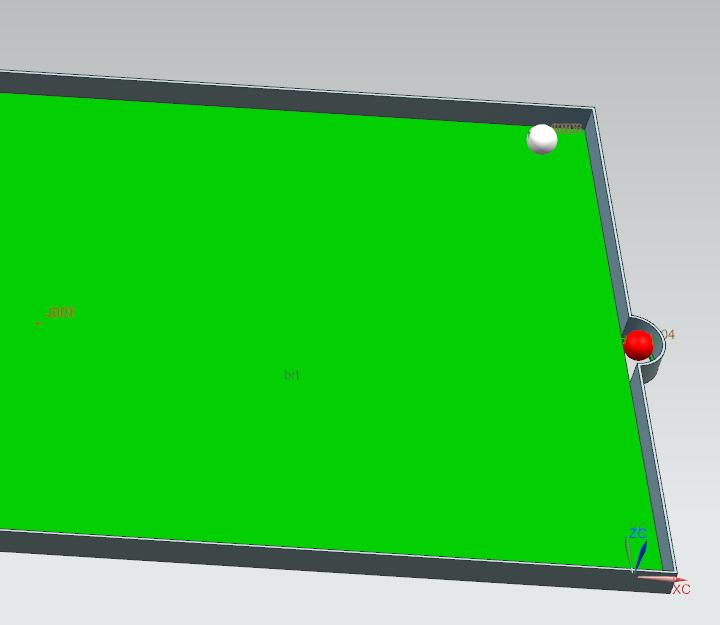
\includegraphics[height=5cm,width=1\textwidth,keepaspectratio]{var7_4.jpeg}
			\caption{}
			\label{fig:var7_4.jpeg}
		\end{subfigure}
	\end{figure}
}

\ttask{Spring clamp}{
	Construct a geometrical model of the simple mechanism shown in \cref{fig:var8_0.jpeg,fig:var8_1.jpeg}. 
	- The idea of the mechanism is that the blue platform under the action of the applied momentum begins to rotate around the fixed gray base. The speed of rotation gradually increases. The green cross, is connected to the blue platform by a kinematic pair of the Slider type. The green cross is connected to the gray base by two red spring-loaded brackets (rotary joints, \cref{fig:var8_1.jpeg}).

	The parameters are following:
	\begin{itemize}
		\item Green cross weight: 10 kg.
		\item Set the applied torque so that the angular rotation speed of the blue platform around the gray base increases in about 1 second from 0 to 2 revolute per sec.
		\item Elasticity coefficient of the springs is 20 N/mm.
	\end{itemize}
}{
	\begin{itemize}
		\item Under the action of centrifugal force the green cross is gradually detached from the gray base (\cref{fig:var8_2.jpeg,fig:var8_3.jpeg,fig:var8_4.jpeg,fig:var8_5.jpeg,fig:var8_6.jpeg}). Analyze the process of detachment. Plot the angular velocity of the blue platform.
		\item Plot the change in the distance between the ends of the red staples.
	\end{itemize}

	\begin{figure}[H]
		\begin{subfigure}{0.49\textwidth}
			\centering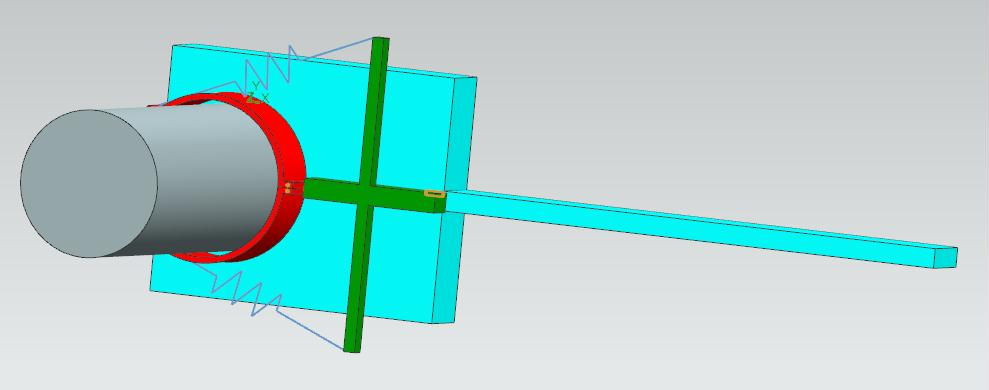
\includegraphics[height=6cm,width=1\textwidth,keepaspectratio]{var8_0.jpeg}
			\caption{}
			\label{fig:var8_0.jpeg}
		\end{subfigure}
		\begin{subfigure}{0.49\textwidth}
			\centering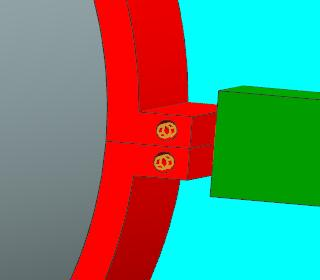
\includegraphics[height=6cm,width=1\textwidth,keepaspectratio]{var8_1.jpeg}
			\caption{}
			\label{fig:var8_1.jpeg}
		\end{subfigure}

		\begin{subfigure}{0.19\textwidth}
			\centering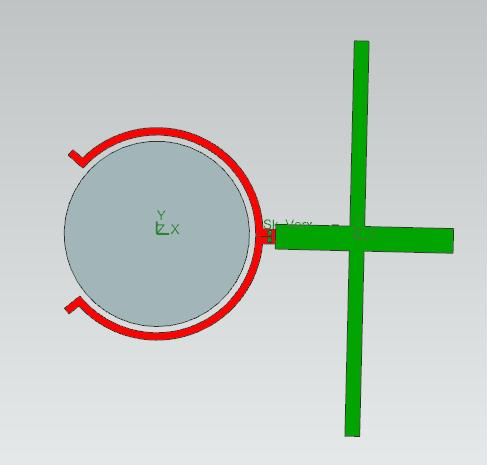
\includegraphics[height=6cm,width=1\textwidth,keepaspectratio]{var8_2.jpeg}
			\caption{}
			\label{fig:var8_2.jpeg}
		\end{subfigure}
	\begin{subfigure}{0.19\textwidth}
		\centering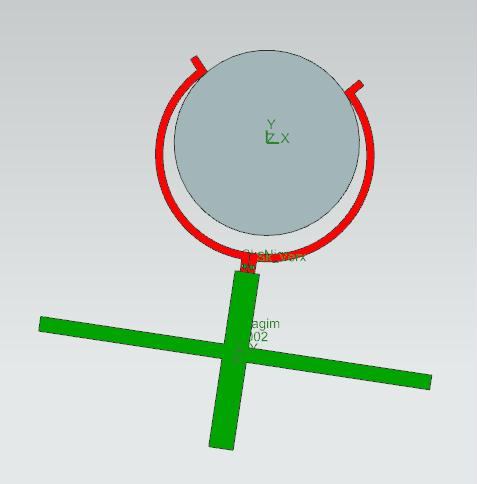
\includegraphics[height=6cm,width=1\textwidth,keepaspectratio]{var8_3.jpeg}
		\caption{}
		\label{fig:var8_3.jpeg}
	\end{subfigure}
	\begin{subfigure}{0.19\textwidth}
		\centering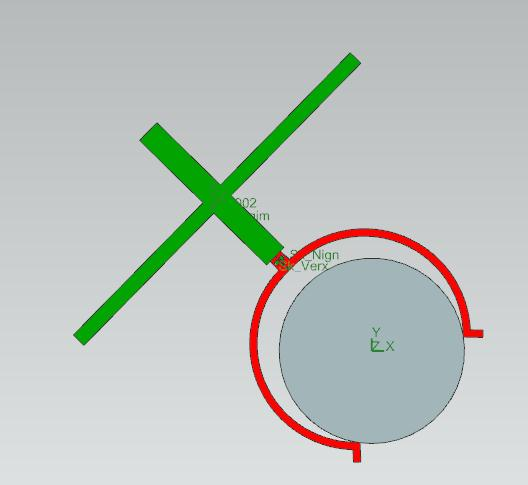
\includegraphics[height=6cm,width=1\textwidth,keepaspectratio]{var8_4.jpeg}
		\caption{}
		\label{fig:var8_4.jpeg}
	\end{subfigure}
	\begin{subfigure}{0.19\textwidth}
		\centering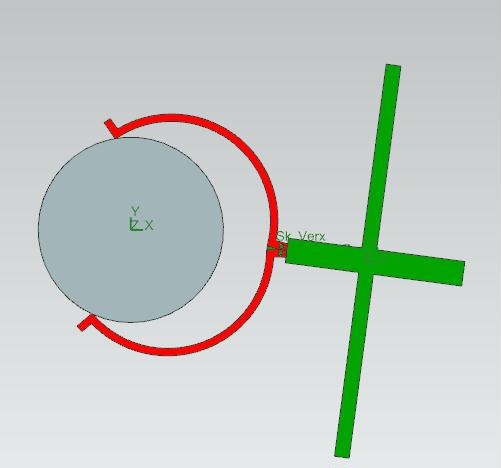
\includegraphics[height=6cm,width=1\textwidth,keepaspectratio]{var8_5.jpeg}
		\caption{}
		\label{fig:var8_5.jpeg}
	\end{subfigure}
	\begin{subfigure}{0.19\textwidth}
		\centering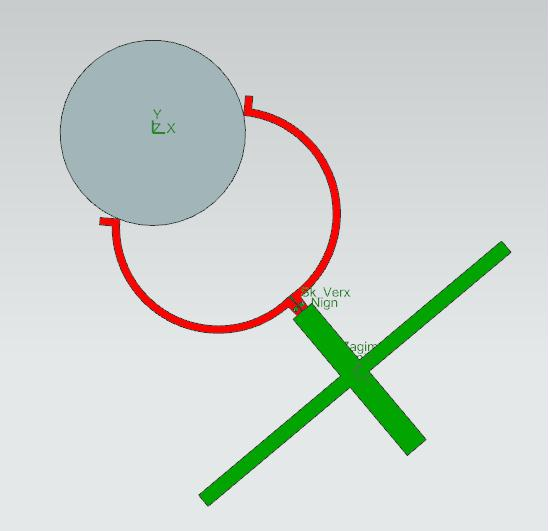
\includegraphics[height=6cm,width=1\textwidth,keepaspectratio]{var8_6.jpeg}
		\caption{}
		\label{fig:var8_6.jpeg}
	\end{subfigure}
	\end{figure}
}

\ttask{Gymnast}{
	Construct a geometric model of the system: the person on the bar. Make sure that the masses of individual parts of the human body are real (torso - 80 kg, arm - 7 kg, leg - 14 kg, etc.). The initial position is almost horizontal to the ground (\cref{fig:var9_0.jpeg}).
}{
	\begin{itemize}
		\item At first, simulate the free swing of the "gymnast" only under the action of your own weight.
		\item Then select the amount of additional torque the "gymnast" must generate in order to make a complete turn around the bar (\cref{fig:var9_0.jpeg,fig:var9_1.jpeg,fig:var9_2.jpeg,fig:var9_3.jpeg,fig:var9_4.jpeg}). 
		\item The amount of torque should be applied only during the first half stroke (\cref{fig:var9_5.jpeg}).
		\item Plot the angular velocity of the "gymnast".
	\end{itemize}

	\begin{figure}[H]
		\begin{subfigure}{0.32\textwidth}
			\centering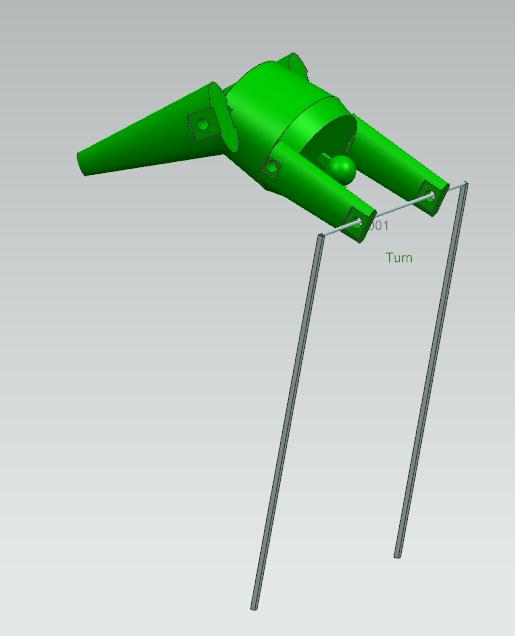
\includegraphics[height=6cm,width=1\textwidth,keepaspectratio]{var9_0.jpeg}
			\caption{}
			\label{fig:var9_0.jpeg}
		\end{subfigure}
		\begin{subfigure}{0.32\textwidth}
			\centering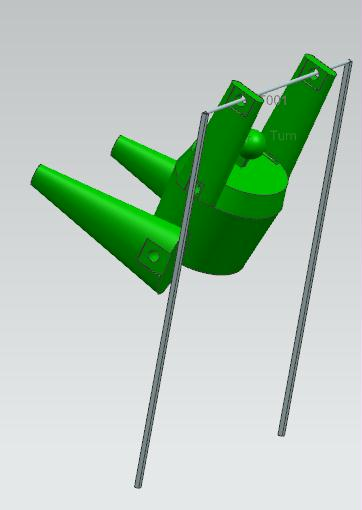
\includegraphics[height=6cm,width=1\textwidth,keepaspectratio]{var9_1.jpeg}
			\caption{}
			\label{fig:var9_1.jpeg}
		\end{subfigure}
		\begin{subfigure}{0.32\textwidth}
			\centering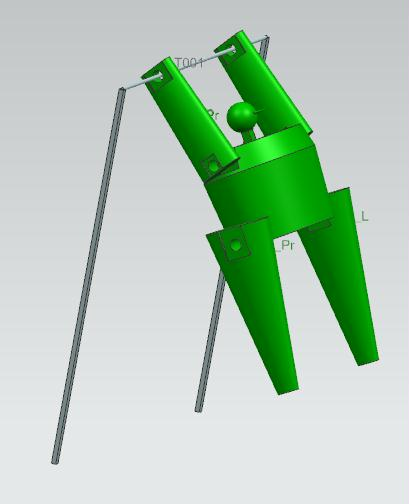
\includegraphics[height=6cm,width=1\textwidth,keepaspectratio]{var9_2.jpeg}
			\caption{}
			\label{fig:var9_2.jpeg}
		\end{subfigure}
	
		\begin{subfigure}{0.32\textwidth}
			\centering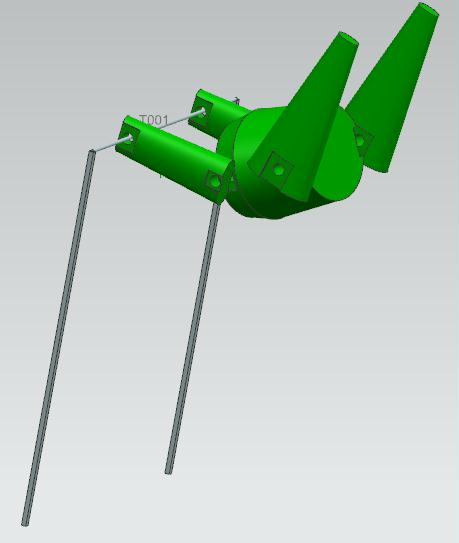
\includegraphics[height=6cm,width=1\textwidth,keepaspectratio]{var9_3.jpeg}
			\caption{}
			\label{fig:var9_3.jpeg}
		\end{subfigure}
		\begin{subfigure}{0.32\textwidth}
			\centering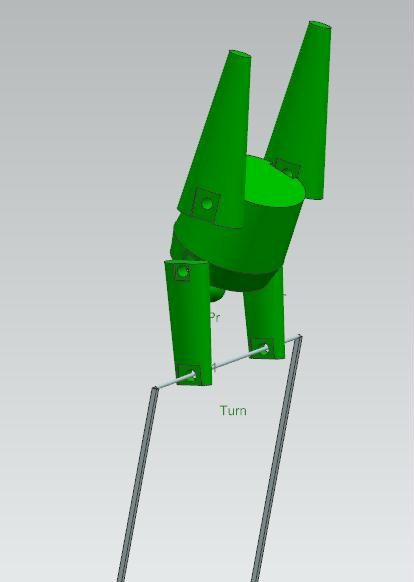
\includegraphics[height=6cm,width=1\textwidth,keepaspectratio]{var9_4.jpeg}
			\caption{}
			\label{fig:var9_4.jpeg}
		\end{subfigure}
		\begin{subfigure}{0.32\textwidth}
			\centering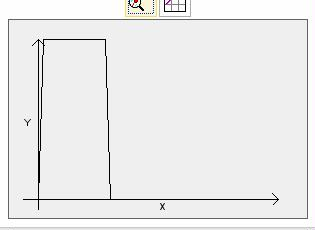
\includegraphics[height=6cm,width=1\textwidth,keepaspectratio]{var9_5.jpeg}
			\caption{}
			\label{fig:var9_5.jpeg}
		\end{subfigure}
	\end{figure}
}

\ttask{Backflip}{
	Construct a geometric model of the system: a man on a uneven surface (\cref{fig:var10_0.jpeg}). Make sure that the masses of individual parts of the human body are real (torso - 80 kg, arm - 7 kg, leg - 14 kg, etc.). Initial position is to be ready to do a backflip (\cref{fig:var10_0.jpeg}).
}{
	\begin{itemize}
		\item Use a combination of forces and torques acting for a short time (\cref{sub@fig:var10_6.jpeg}) on the "gymnast" to simulate his attempt to do a backflip (\cref{fig:var10_0.jpeg,fig:var10_1.jpeg,fig:var10_2.jpeg,fig:var10_3.jpeg,fig:var10_4.jpeg,fig:var10_5.jpeg}).
	\end{itemize}

	\begin{figure}[H]
		\begin{subfigure}{0.32\textwidth}
			\centering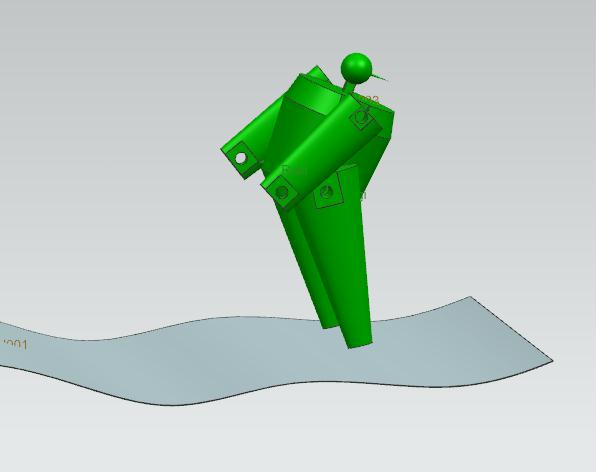
\includegraphics[height=6cm,width=1\textwidth,keepaspectratio]{var10_0.jpeg}
			\caption{}
			\label{fig:var10_0.jpeg}
		\end{subfigure}
		\begin{subfigure}{0.32\textwidth}
			\centering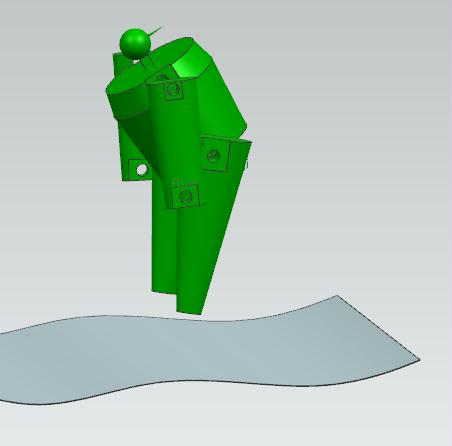
\includegraphics[height=6cm,width=1\textwidth,keepaspectratio]{var10_1.jpeg}
			\caption{}
			\label{fig:var10_1.jpeg}
		\end{subfigure}
		\begin{subfigure}{0.32\textwidth}
			\centering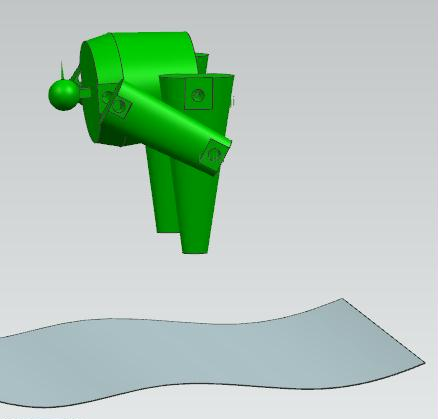
\includegraphics[height=6cm,width=1\textwidth,keepaspectratio]{var10_2.jpeg}
			\caption{}
			\label{fig:var10_2.jpeg}
		\end{subfigure}
	
		\begin{subfigure}{0.24\textwidth}
			\centering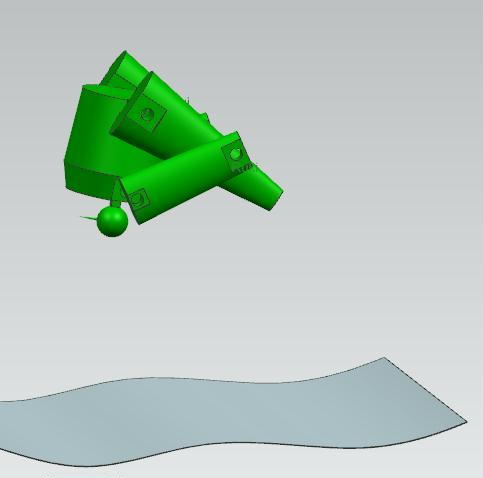
\includegraphics[height=6cm,width=1\textwidth,keepaspectratio]{var10_3.jpeg}
			\caption{}
			\label{fig:var10_3.jpeg}
		\end{subfigure}
		\begin{subfigure}{0.24\textwidth}
			\centering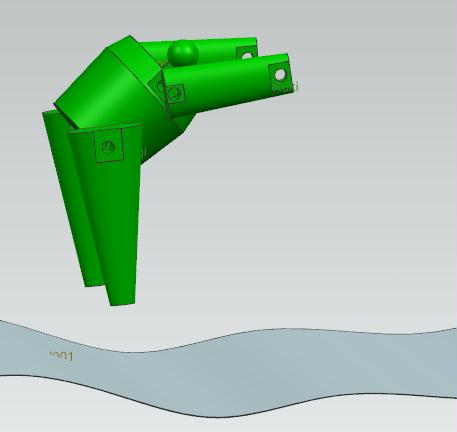
\includegraphics[height=6cm,width=1\textwidth,keepaspectratio]{var10_4.jpeg}
			\caption{}
			\label{fig:var10_4.jpeg}
		\end{subfigure}
		\begin{subfigure}{0.24\textwidth}
			\centering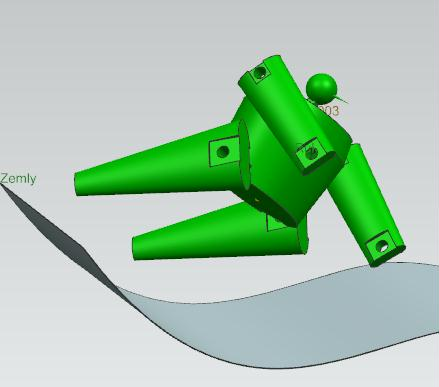
\includegraphics[height=6cm,width=1\textwidth,keepaspectratio]{var10_5.jpeg}
			\caption{}
			\label{fig:var10_5.jpeg}
		\end{subfigure}
		\begin{subfigure}{0.24\textwidth}
			\centering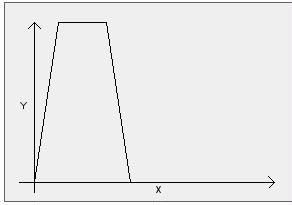
\includegraphics[height=6cm,width=1\textwidth,keepaspectratio]{var10_6.jpeg}
			\caption{}
			\label{fig:var10_6.jpeg}
		\end{subfigure}
	\end{figure}	
}

\end{document} % This is the end of the document